\thispagestyle{empty}
\refstepcounter{dummy}

\pdfbookmark[1]{Annexes}{Annexes} % Bookmark name visible in a PDF viewer

\addcontentsline{toc}{chapter}{Annexes}
\vspace*{3cm}

\chapter*{Annexes}
\label{appendix} 


\begin{figure}[H]
    \centering
    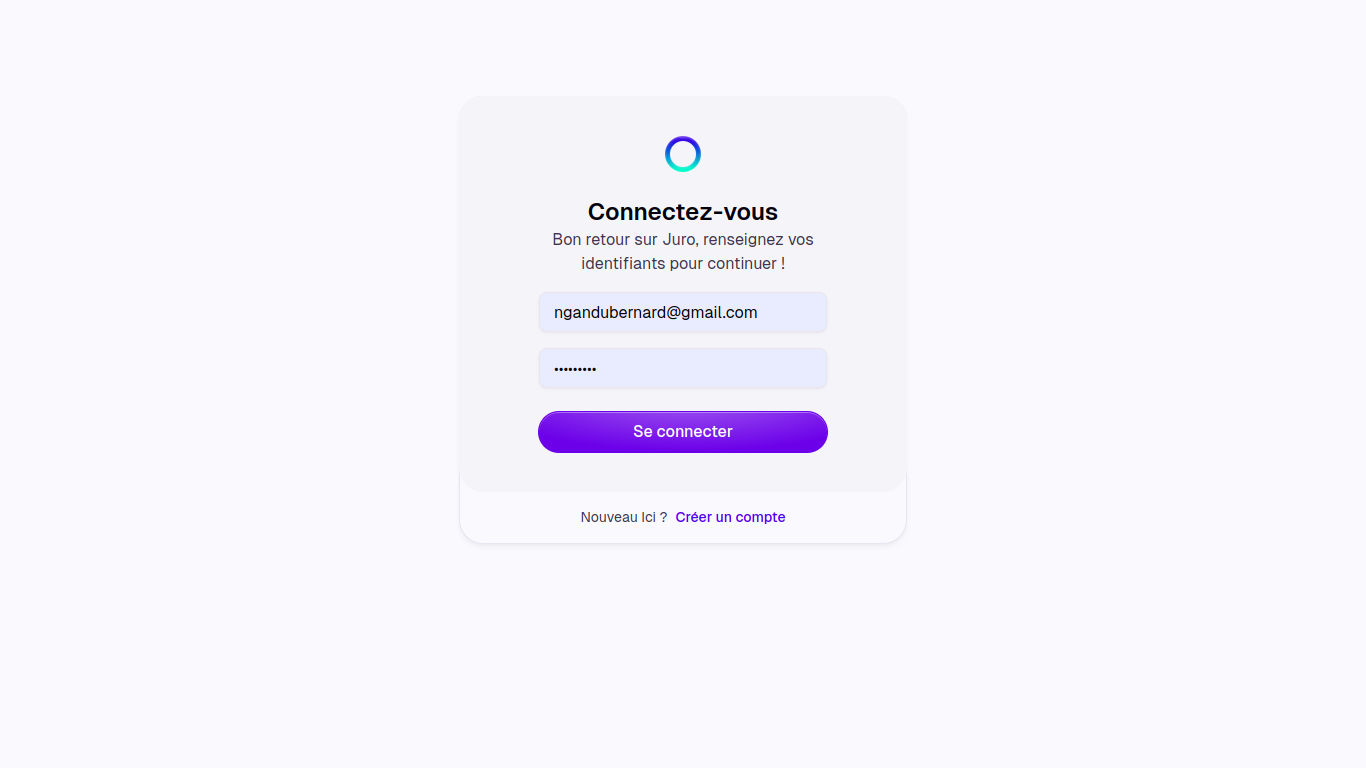
\includegraphics[width=15cm]{Images/screenshot-juro-1.png}
    \caption{Capture d'écran page de connexion}
    \label{fig:app-screenshot-1}
\end{figure}

\begin{figure}[H]
    \centering
    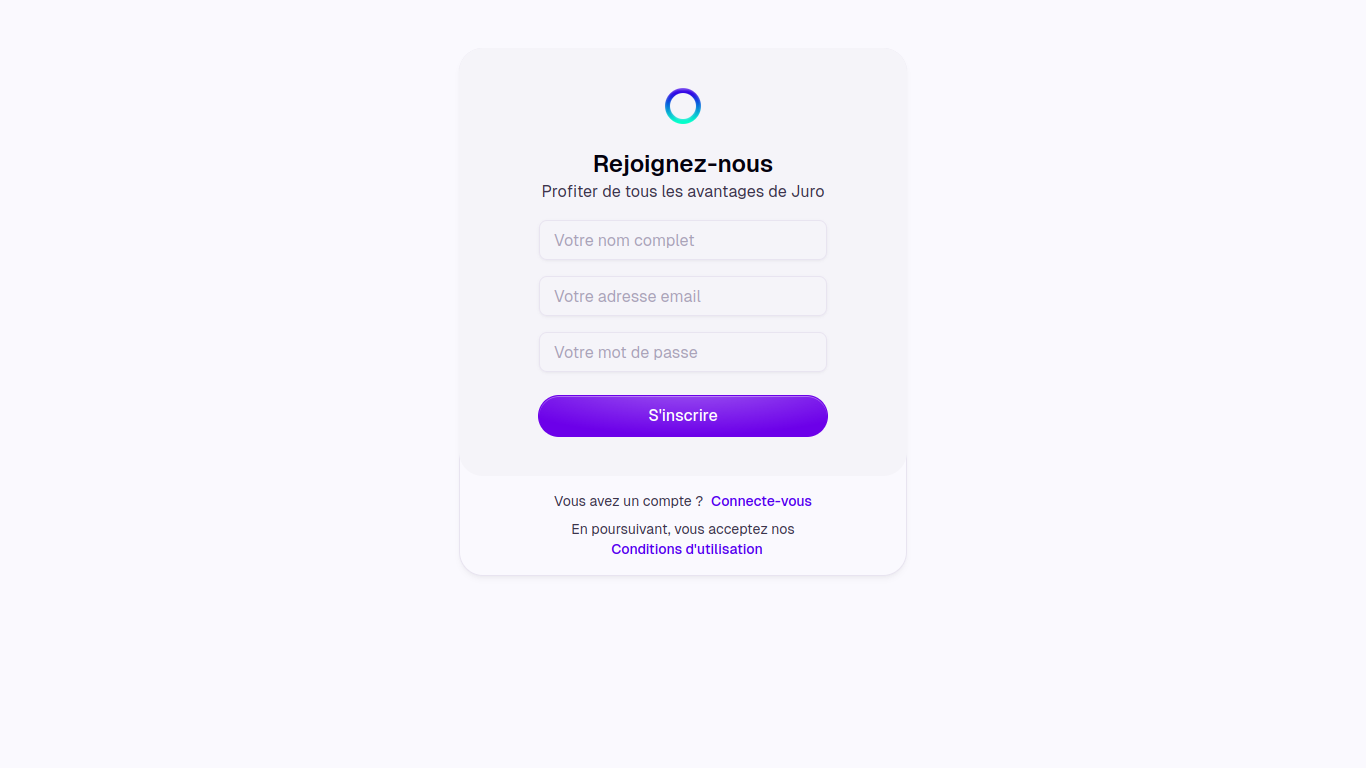
\includegraphics[width=15cm]{Images/screenshot-juro-2.png}
    \caption{Capture d'écran page d'inscription}
    \label{fig:app-screenshot-1}
\end{figure}

\begin{figure}[H]
    \centering
    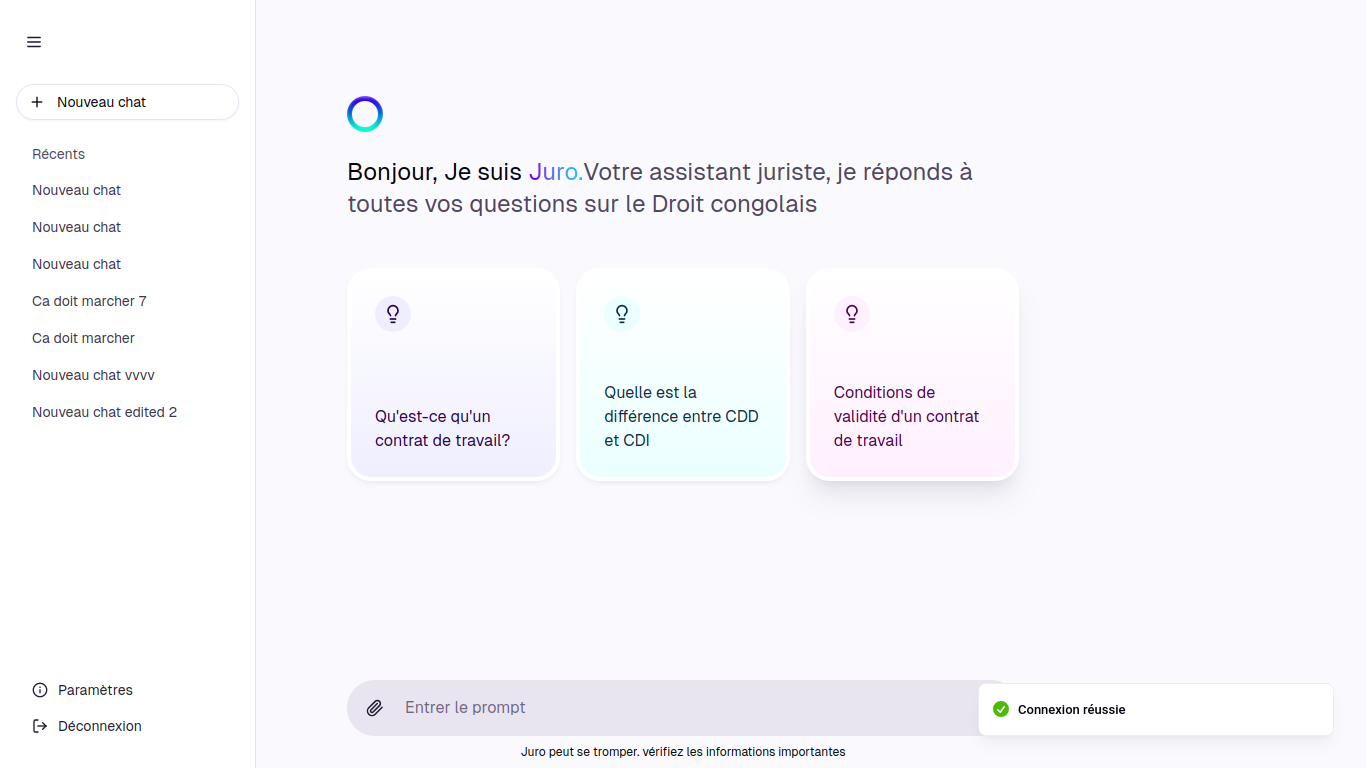
\includegraphics[width=15cm]{Images/screenshot-juro-3.png}
    \caption{Capture d'écran page de chat}
    \label{fig:app-screenshot-1}
\end{figure}

\begin{figure}[H]
    \centering
    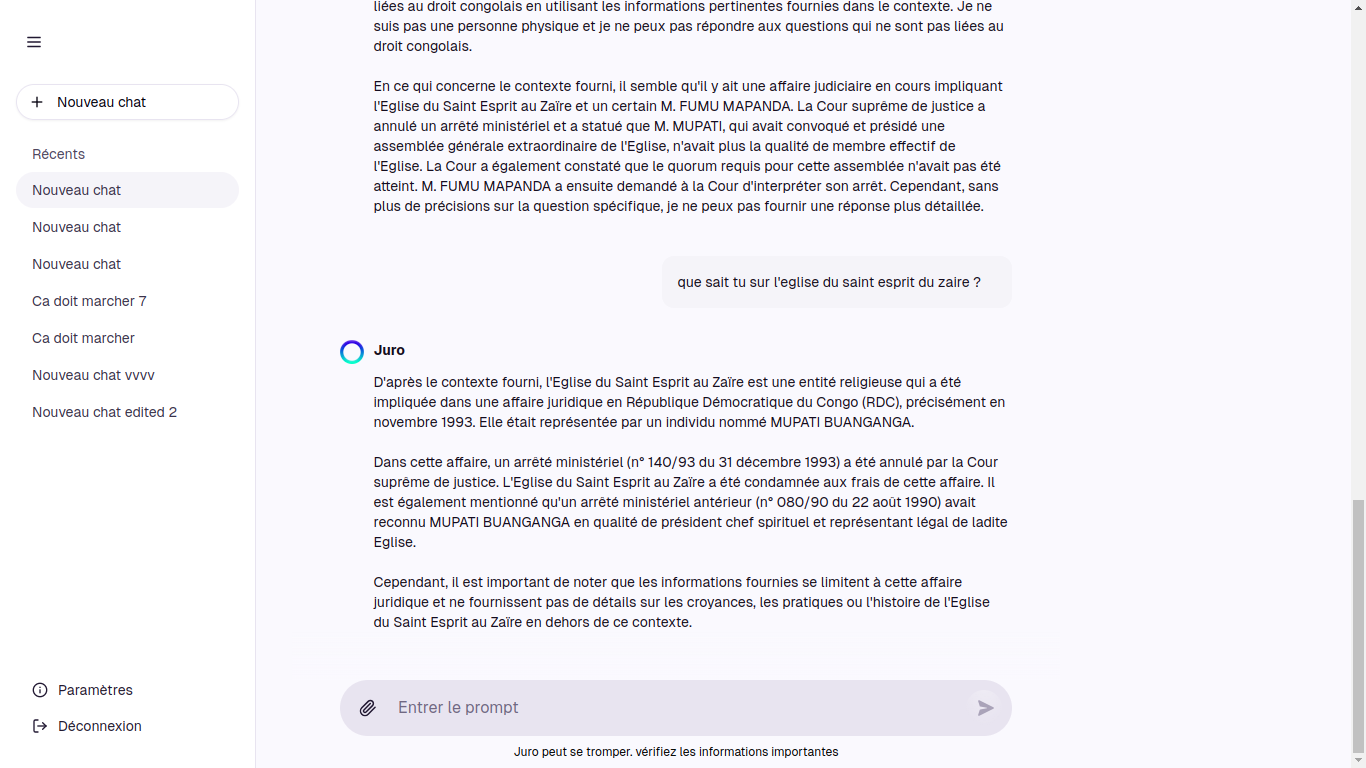
\includegraphics[width=15cm]{Images/screenshot-juro-4.png}
    \caption{Capture d'écran page lecture de message}
    \label{fig:app-screenshot-1}
\end{figure}

\begin{figure}[H]
    \centering
    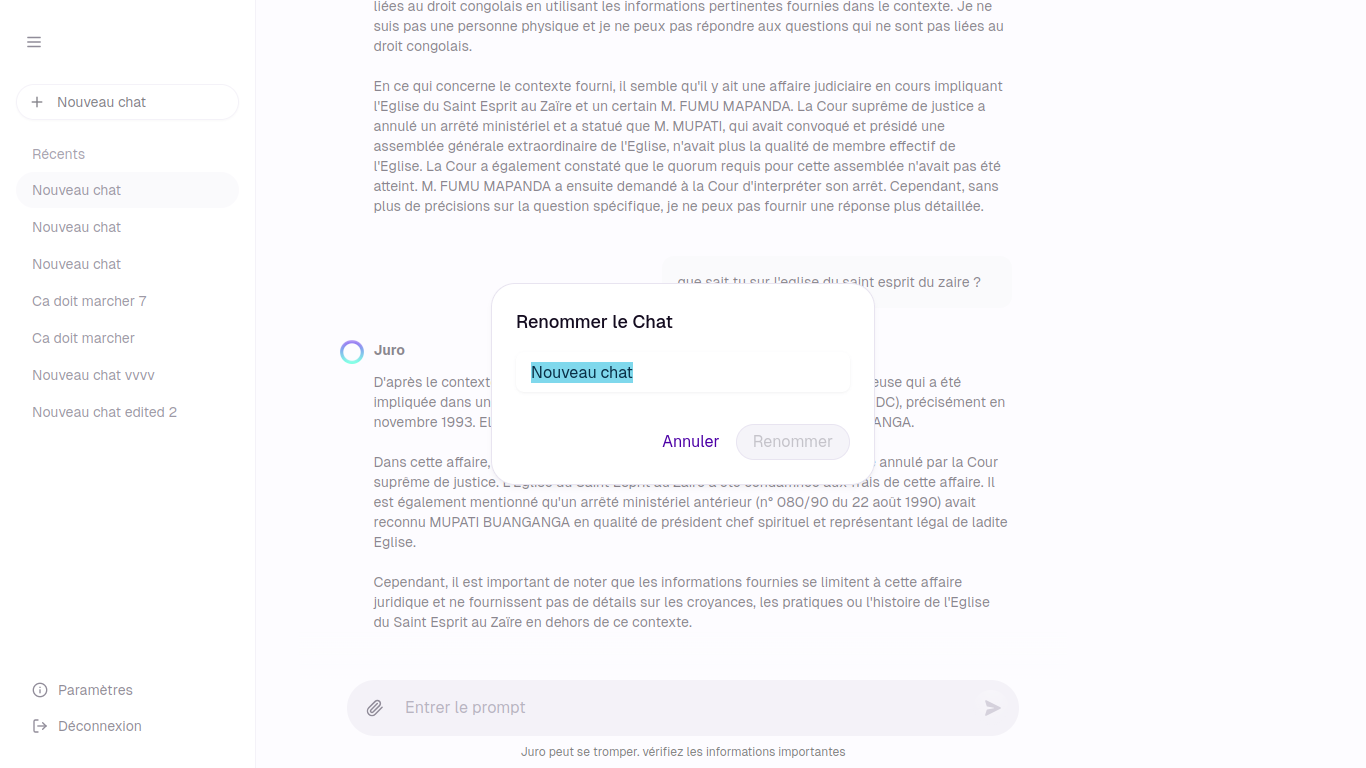
\includegraphics[width=15cm]{Images/screenshot-juro-5.png}
    \caption{Capture d'écran modifier le chat}
    \label{fig:app-screenshot-1}
\end{figure}

\begin{figure}[H]
    \centering
    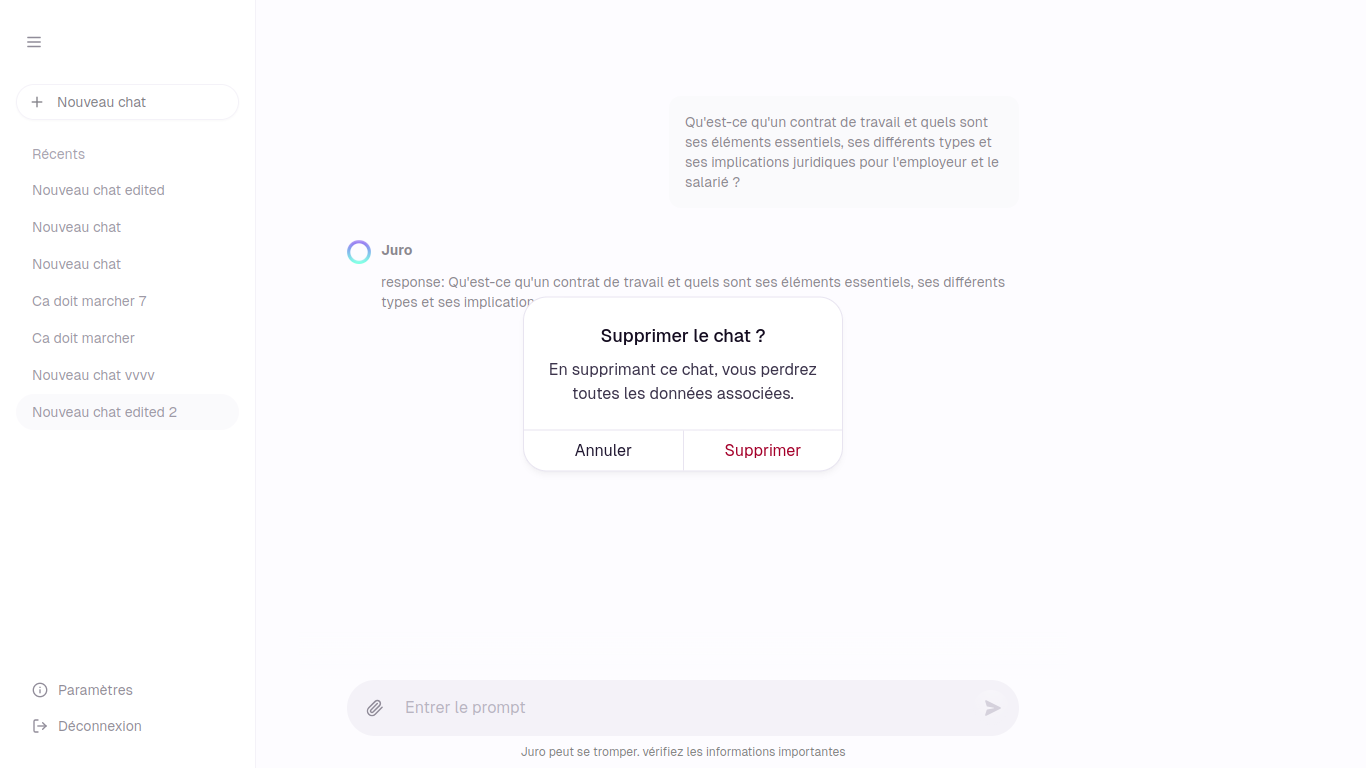
\includegraphics[width=15cm]{Images/screenshot-juro-6.png}
    \caption{Capture d'écran supprimer le chat}
    \label{fig:app-screenshot-1}
\end{figure}

\begin{listing}[!ht]
\begin{minted}{python}
# Extract images and use OCR if necessary
image_list = page.get_images(full=True)
for image_index, img in enumerate(page.get_images(full=True)):
    xref = img[0]
    # Extract the image bytes
    base_image = doc.extract_image(xref)
    image_bytes = base_image["image"]
    image = Image.open(io.BytesIO(image_bytes))
    ocr_text = pytesseract.image_to_string(
        image, 
        lang='eng',
        output_type=Output.STRING
    )
    
    extracted_content.append({
        'page': page_num + 1, 
        'type': 'image', 
        'content': ocr_text, 
        'image_index': image_index + 1
    })
\end{minted}
\caption{Extraction avec OCR sur les images}
\label{appendix:code:python:text-extract-images}
\end{listing}

\begin{listing}[!ht]
\begin{minted}{python}
import matplotlib.pyplot as plt

years = [
    '2010', '2011', '2012', '2013', '2014', '2015', '2016', '2017', 
    '2018*', '2019*', '2020*', '2021*', '2022*', '2023*', '2024*', '2025*'
]
values = [2, 5, 6.5, 9, 12.5, 15.5, 18, 26, 33, 41, 64.2, 79, 97, 120, 147, 181]

fig, ax = plt.subplots(figsize=(12, 6), dpi=100)
ax.spines['right'].set_visible(False)
ax.spines['top'].set_visible(False)
ax.spines['left'].set_visible(False)

plt.grid(alpha=0.3, zorder=0, linestyle='dashed', axis='y')
bars = plt.bar(
    years, values, hatch="/", color="#9ca3af", 
    edgecolor="#374151", alpha=0.8, width=0.8, zorder=3
)

for bar in bars:
    yval = bar.get_height()
    plt.text(
        bar.get_x() + bar.get_width()/2, yval + 5, 
        round(yval, 1), ha='center', va='bottom', fontweight="bold"
    )

plt.ylabel('Data Volume in Zettabytes', fontweight="bold")
plt.show()
\end{minted}
\caption{Code python utilisé pour générer la figure \ref{fig:datagenerated}}
\label{appendix:code:python:plot-generation}
\end{listing}

\begin{listing}[!ht]
\begin{minted}{python}
import numpy as np
import matplotlib.pyplot as plt
from mpl_toolkits.mplot3d import Axes3D

# Fonction à minimiser
def f(x, y):
    return x**2 + y**2

# Gradient de la fonction
def grad_f(x, y):
    return np.array([2*x, 2*y])

# Paramètres de descente de gradient
alpha = 0.1 # taux d'apprentissage
n_iterations = 10
x_start = np.array([0.8, 0.8]) # point de départ

# Descente de gradient
points = [x_start]
for _ in range(n_iterations):
    grad = grad_f(*points[-1])
    new_point = points[-1] - alpha * grad
    points.append(new_point)

points = np.array(points)

# Création de la grille pour le graphique
x = np.linspace(-1, 1, 400)
y = np.linspace(-1, 1, 400)
x, y = np.meshgrid(x, y)
z = f(x, y)

# Plot 3D
fig = plt.figure(figsize=(14, 9))
ax = fig.add_subplot(111, projection='3d')
ax.plot_surface(x, y, z, alpha=0.5, cmap='winter', edgecolor='none')
ax.scatter(points[:, 0], points[:, 1], f(points[:, 0], points[:, 1]), color='red', s=50)
ax.view_init(45, 280)
ax.set_xlabel('X', fontweight="bold")
ax.set_ylabel('Y', fontweight="bold")
ax.set_zlabel('f(X, Y)', fontweight="bold")

plt.show()
\end{minted}
\caption{Code python utilisé pour générer la figure \ref{fig:gradient-descent}}
\label{appendix:code:python:gd}
\end{listing}


\begin{listing}[!ht]
\begin{minted}{python}
import os
import hashlib
from tqdm import tqdm

def calculate_md5(file_path):
    """Calculate the MD5 hash of a file."""
    hash_md5 = hashlib.md5()
    with open(file_path, 'rb') as f:
        for chunk in iter(lambda: f.read(4096), b""):
            hash_md5.update(chunk)
    return hash_md5.hexdigest()

def rename_files_in_directory(directory_path):
    """Rename each file in the directory to its MD5 hash."""
    files = [
        f for f in os.listdir(directory_path) 
        if not os.path.isdir(os.path.join(directory_path, f))
    ]
    
    for filename in tqdm(files, desc="Renaming files"):
        file_path = os.path.join(directory_path, filename)
        md5_hash = calculate_md5(file_path)
        new_file_name = md5_hash
        new_file_path = os.path.join(directory_path, new_file_name)
        os.rename(file_path, new_file_path)


directory_path = '/content/drive/MyDrive/DATA/LawLLM/PDF/'
rename_files_in_directory(directory_path)
\end{minted}
\caption{Script python permettant de renommer un fichier par son hash MD5}
\label{appendix:code:python:md5-filename-hashing}
\end{listing}

\begin{listing}[!ht]
\begin{minted}{python}
import os
from openai import OpenAI
import pandas as pd

questions = pd.read_csv('_magistrature.csv')
client = OpenAI(api_key=os.getenv('OPENAI_KEY'))

def generate_content(x):
    print(f"Answering question: {x['question']}")
    prompt = f"""
        Dans le contexte du Droit Congolais (RDC) précisément {x['category']},
        répondez à la question suivante : {x['question']}
    """

    completion = client.chat.completions.create(
        model="gpt-3.5-turbo",
        messages=[
            {
                "role": "system",
                "content": """
                    Tu es un assistant virtuel qui peut répondre 
                    à des questions sur le droit congolais (RDC).
                """
            },
            {"role": "user", "content": prompt}
        ]
    )
    return completion.choices[0].message.content

questions['model'] = 'gpt-3.5-turbo'
questions['answer'] = questions.apply(lambda x: generate_content(x), axis=1)
questions.to_csv('./data/answers-gpt-3.5-turbo.csv', index=False)
\end{minted}
\caption{Évalutation des modèles OpenAI sur le test de magistrature 2022.}
\label{appendix:code:python:gpt-3-evaluation}
\end{listing}

\begin{listing}[!ht]
\begin{minted}{python}
import matplotlib.pyplot as plt

years = ['gpt3.5-turbo', 'gemini-pro', 'llama2', 'mistral', 'vicuna']
values = [65.33, 59.20, 43.11, 38.00, 36.44]

fig, ax = plt.subplots(figsize=(12, 6), dpi=100)
ax.spines['right'].set_visible(False)
ax.spines['top'].set_visible(False)
ax.spines['left'].set_visible(False)

plt.grid(alpha=0.3, zorder=0, linestyle='dashed', axis='y')
bars = plt.bar(
    years, 
    values, 
    hatch="/", 
    color="#9ca3af", 
    edgecolor="#374151", 
    alpha=0.8, 
    width=0.8, 
    zorder=3
)

for bar in bars:
    yval = bar.get_height()
    plt.text(
        bar.get_x() + bar.get_width()/2, 
        yval + 5, 
        round(yval, 1), 
        ha='center', 
        va='bottom', 
        fontweight="bold"
    )

plt.ylabel('Résultat au test (en pourcentage)', fontweight="bold")
plt.show()
\end{minted}
\caption{Code python utilisé pour générer la figure \ref{fig:model-result}}
\label{appendix:code:python:model-result}
\end{listing}
